\documentclass[12pt,reqno]{article}
\usepackage{amsthm, amsmath, amsfonts, amssymb, amscd, mathtools, youngtab, euscript, mathrsfs, verbatim, enumerate, multicol, multirow, bbding, color, babel, esint, geometry, tikz, tikz-cd, tikz-3dplot, array, enumitem, hyperref, thm-restate, thmtools, datetime, graphicx, tensor, braket, slashed, standalone, pgfplots, ytableau, subfigure, wrapfig, dsfont, setspace, wasysym, pifont, float, rotating, adjustbox, pict2e,array}
\usepackage{amsmath}
\usepackage[utf8]{inputenc}
\usetikzlibrary{arrows, positioning, decorations.pathmorphing, decorations.pathreplacing, decorations.markings, matrix, patterns}
\tikzset{big arrow/.style={
    decoration={markings,mark=at position 1 with {\arrow[scale=1.5,#1]{>}}},
    postaction={decorate},
    shorten >=0.4pt},
  big arrow/.default=black}

\begin{document}

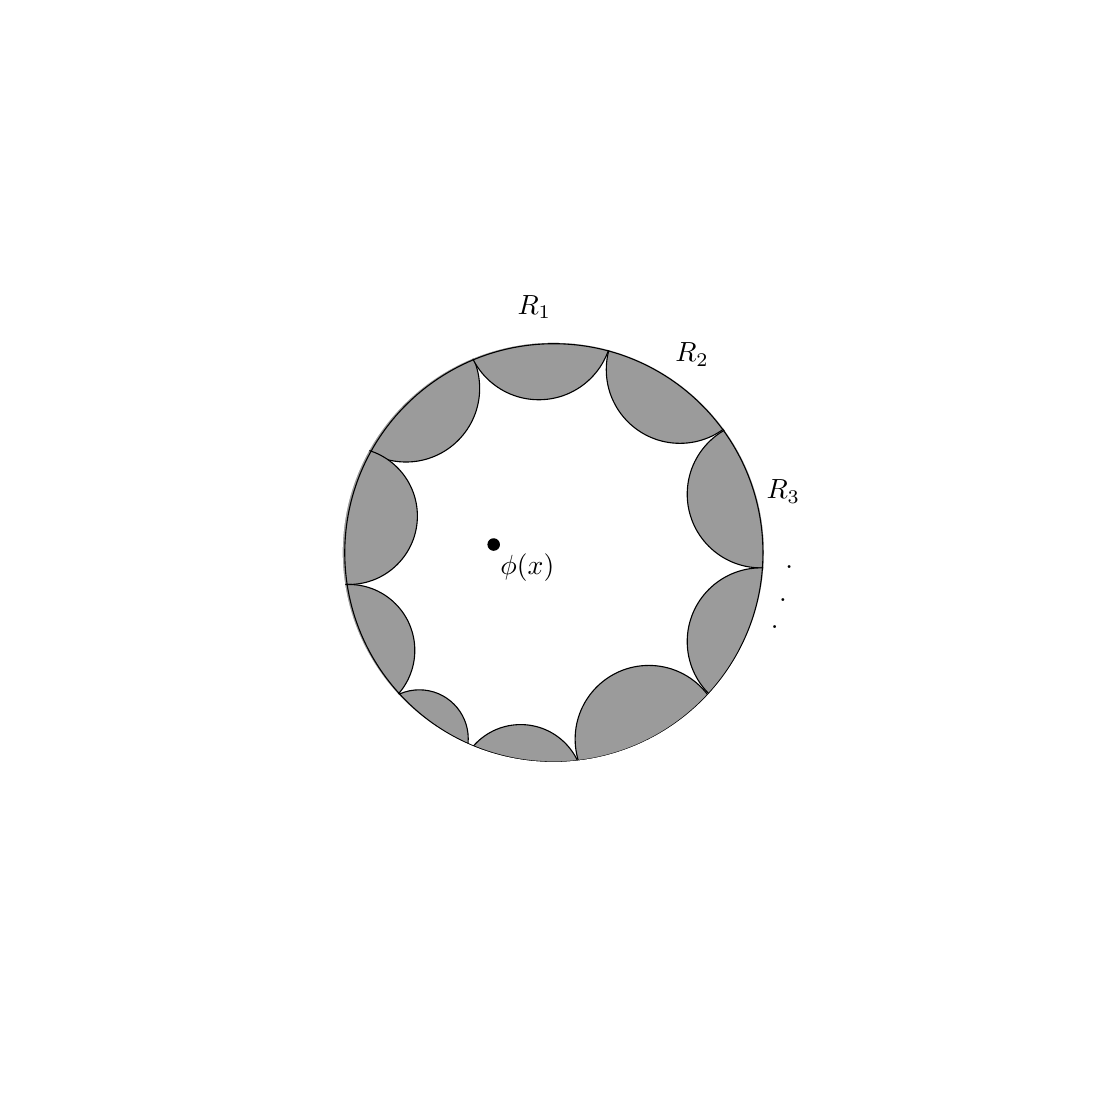
\begin{tikzpicture}[x=0.75pt,y=0.75pt,yscale=-1,xscale=1]
\draw  [fill={rgb, 255:red, 155; green, 155; blue, 155 }  ,fill opacity=1 ] (228,60.5) .. controls (228,40.89) and (243.89,25) .. (263.5,25) .. controls (283.11,25) and (299,40.89) .. (299,60.5) .. controls (299,80.11) and (283.11,96) .. (263.5,96) .. controls (243.89,96) and (228,80.11) .. (228,60.5) -- cycle ;
\draw    (536.5,146) .. controls (557.5,129) and (557.5,84) .. (523.5,73) ;
\draw  [fill={rgb, 255:red, 155; green, 155; blue, 155 }  ,fill opacity=1 ] (203,122) .. controls (203,103.77) and (217.77,89) .. (236,89) .. controls (254.23,89) and (269,103.77) .. (269,122) .. controls (269,140.23) and (254.23,155) .. (236,155) .. controls (217.77,155) and (203,140.23) .. (203,122) -- cycle ;
\draw  [fill={rgb, 255:red, 155; green, 155; blue, 155 }  ,fill opacity=1 ] (292,30.5) .. controls (292,10.89) and (307.89,-5) .. (327.5,-5) .. controls (347.11,-5) and (363,10.89) .. (363,30.5) .. controls (363,50.11) and (347.11,66) .. (327.5,66) .. controls (307.89,66) and (292,50.11) .. (292,30.5) -- cycle ;
\draw  [fill={rgb, 255:red, 155; green, 155; blue, 155 }  ,fill opacity=1 ] (360,51.5) .. controls (360,31.89) and (375.89,16) .. (395.5,16) .. controls (415.11,16) and (431,31.89) .. (431,51.5) .. controls (431,71.11) and (415.11,87) .. (395.5,87) .. controls (375.89,87) and (360,71.11) .. (360,51.5) -- cycle ;
\draw  [fill={rgb, 255:red, 155; green, 155; blue, 155 }  ,fill opacity=1 ] (399,111.5) .. controls (399,91.89) and (414.89,76) .. (434.5,76) .. controls (454.11,76) and (470,91.89) .. (470,111.5) .. controls (470,131.11) and (454.11,147) .. (434.5,147) .. controls (414.89,147) and (399,131.11) .. (399,111.5) -- cycle ;
\draw  [fill={rgb, 255:red, 155; green, 155; blue, 155 }  ,fill opacity=1 ] (399,182.5) .. controls (399,162.89) and (414.89,147) .. (434.5,147) .. controls (454.11,147) and (470,162.89) .. (470,182.5) .. controls (470,202.11) and (454.11,218) .. (434.5,218) .. controls (414.89,218) and (399,202.11) .. (399,182.5) -- cycle ;
\draw  [fill={rgb, 255:red, 155; green, 155; blue, 155 }  ,fill opacity=1 ] (345,229.5) .. controls (345,209.89) and (360.89,194) .. (380.5,194) .. controls (400.11,194) and (416,209.89) .. (416,229.5) .. controls (416,249.11) and (400.11,265) .. (380.5,265) .. controls (360.89,265) and (345,249.11) .. (345,229.5) -- cycle ;
\draw  [fill={rgb, 255:red, 155; green, 155; blue, 155 }  ,fill opacity=1 ] (288.5,252.75) .. controls (288.5,236.04) and (302.04,222.5) .. (318.75,222.5) .. controls (335.46,222.5) and (349,236.04) .. (349,252.75) .. controls (349,269.46) and (335.46,283) .. (318.75,283) .. controls (302.04,283) and (288.5,269.46) .. (288.5,252.75) -- cycle ;
\draw  [fill={rgb, 255:red, 155; green, 155; blue, 155 }  ,fill opacity=1 ] (204.25,186.75) .. controls (204.25,169.21) and (218.46,155) .. (236,155) .. controls (253.54,155) and (267.75,169.21) .. (267.75,186.75) .. controls (267.75,204.29) and (253.54,218.5) .. (236,218.5) .. controls (218.46,218.5) and (204.25,204.29) .. (204.25,186.75) -- cycle ;
\draw  [fill={rgb, 255:red, 155; green, 155; blue, 155 }  ,fill opacity=1 ] (246.38,229.31) .. controls (246.38,216.3) and (256.92,205.75) .. (269.94,205.75) .. controls (282.95,205.75) and (293.5,216.3) .. (293.5,229.31) .. controls (293.5,242.33) and (282.95,252.88) .. (269.94,252.88) .. controls (256.92,252.88) and (246.38,242.33) .. (246.38,229.31) -- cycle ;
\draw   (234,139.75) .. controls (234,84.11) and (279.11,39) .. (334.75,39) .. controls (390.39,39) and (435.5,84.11) .. (435.5,139.75) .. controls (435.5,195.39) and (390.39,240.5) .. (334.75,240.5) .. controls (279.11,240.5) and (234,195.39) .. (234,139.75) -- cycle ;
\draw  [draw opacity=0][fill={rgb, 255:red, 255; green, 255; blue, 255 }  ,fill opacity=1 ,even odd rule] (233,139.5) .. controls (233,83.72) and (278.44,38.5) .. (334.5,38.5) .. controls (390.56,38.5) and (436,83.72) .. (436,139.5) .. controls (436,195.28) and (390.56,240.5) .. (334.5,240.5) .. controls (278.44,240.5) and (233,195.28) .. (233,139.5)(81.5,139.5) .. controls (81.5,0.05) and (194.77,-113) .. (334.5,-113) .. controls (474.23,-113) and (587.5,0.05) .. (587.5,139.5) .. controls (587.5,278.95) and (474.23,392) .. (334.5,392) .. controls (194.77,392) and (81.5,278.95) .. (81.5,139.5) ;
\draw  [fill={rgb, 255:red, 0; green, 0; blue, 0 }  ,fill opacity=1 ] (303,135.75) .. controls (303,134.23) and (304.23,133) .. (305.75,133) .. controls (307.27,133) and (308.5,134.23) .. (308.5,135.75) .. controls (308.5,137.27) and (307.27,138.5) .. (305.75,138.5) .. controls (304.23,138.5) and (303,137.27) .. (303,135.75) -- cycle ;
% Text Node
\draw (316,14.4) node [anchor=north west][inner sep=0.75pt]    {$R_{1}$};
% Text Node
\draw (392,37.4) node [anchor=north west][inner sep=0.75pt]    {$R_{2}$};
% Text Node
\draw (436,103.4) node [anchor=north west][inner sep=0.75pt]    {$R_{3}$};
% Text Node
\draw (445,144.4) node [anchor=north west][inner sep=0.75pt]    {$.$};
% Text Node
\draw (442,160.4) node [anchor=north west][inner sep=0.75pt]    {$.$};
% Text Node
\draw (438,173.4) node [anchor=north west][inner sep=0.75pt]    {$.$};
% Text Node
\draw (307.75,139.15) node [anchor=north west][inner sep=0.75pt]    {$\phi ( x)$};
\end{tikzpicture}

\end{document}